\chapter{Fundamental Algorithms}
\label{chap:fundamental_algorithms}

\begin{figure}[ht]
	\hfill
	\begin{minipage}{0.5\textwidth}
		\centering
		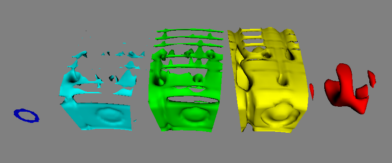
\includegraphics{VTKTextbook-54}\\
		\caption*{\texttt{Isosurfaces of a combustor dataset computed at multiple values..}}
	\end{minipage}
\end{figure}

\firstletter{W}e have seen how to represent basic types of visualization data such as image data, structured grids, unstructured grids, and polygonal data.
This chapter explores methods to transform this data to and from these various representations, eventually generating graphics primitives that we can render.
These methods are called algorithms, and are of special interest to those working in the field of visualization.
Algorithms are the verbs that allow us to express our data in visual form.
By combining these verbs appropriately, we can reduce complex data into simple, readily comprehensible sentences that are the power of data visualization.

\section{Introduction}

The algorithms that transform data are the heart of data visualization.
To describe the various transformations available, we need to categorize algorithms according to the structure and type of transformation.
By structure we mean the effects that transformation has on the topology and geometry of the dataset.
By type we mean the type of dataset that the algorithm operates on.

Structural transformations can be classified in four ways, depending on how they affect the geometry, topology, and attributes of a dataset.

\begin{itemize}

\item \emph{Geometric transformations} alter input geometry but do not changed the topology of the dataset. For example, if we translate, rotate, and/or scale the points of a polygonal dataset, the topology does not change, but the point coordinates, and therefore the geometry, does.

\item \emph{Topological transformations} alter input topology but do not change geometry and attribute data. Converting a dataset type from polygonal data to unstructured grid data, or from image data to unstructured grid, changes the topology but not the geometry. More often, however, the geometry changes whenever the topology does, so topological transformation is uncommon.

\item \emph{Attribute transformations} convert data attributes from one form to another, or create new attributes from the input data. The structure of the dataset remains unaffected. Computing vector magnitude or creating scalars based on elevation are data attribute transformations.

\item \emph{Combined transformations} change both dataset structure and attribute data. For example, computing contour lines or surfaces is a combined transformation.

\end{itemize}

We also may classify algorithms according to the type of data they operate on, or the type of data they generate. By type, we most often mean the type of attribute data, such as scalars or vectors. Typical categories include:

\begin{itemize}

\item \emph{Scalar algorithms} operate on scalar data. For example, the generation of contour lines of temperature on a weather map.

\item \emph{Vector algorithms} operate on vector data. Showing oriented arrows of airflow (direction and magnitude) is an example of vector visualization.

\item \emph{Tensor algorithms} operate on tensor matrices. An example of a tensor algorithm is to show the components of stress or strain in a material using oriented icons.

\item \emph{Modelling algorithms} generate dataset topology or geometry, or surface normals or texture data. Modelling algorithms tend to be the catch-all category for many algorithms, since some do not fit neatly into any single category mentioned above. For example, generating glyphs oriented according to the vector direction and then scaled according to the scalar value, is a combined scalar/vector algorithm. For convenience we classify such an algorithm as a modelling algorithm, because it does not fit squarely into any other category.

\end{itemize}

Algorithms also can be classified according to the type of data they process. This is the most common scheme found in the visualization literature. However, this scheme is not without its problems. Often the categories overlap, resulting in confusion. For example, a category (not mentioned above) is \emph{volume visualization}, which refers to the visualization of volume data (or in our terminology, image data). This category was initially created to describe the visualization of scalar data arranged on a volume, but more recently, vector (and even tensor) data has been visualized on a volume. Hence, we have to qualify our techniques to \emph{volume vector visualization}, or other potentially confusing combinations.

In the text that follows, we will use the attribute type classification scheme: scalar, vector, tensor, and modelling. In cases where the algorithms operate on a particular dataset type, we place them in the appropriate category according to our best judgment. Be forewarned, though, that alternative classification schemes do exist, and may be better suited to describing the true nature of the algorithm.

\begin{figure}[!htb]
	\centering
	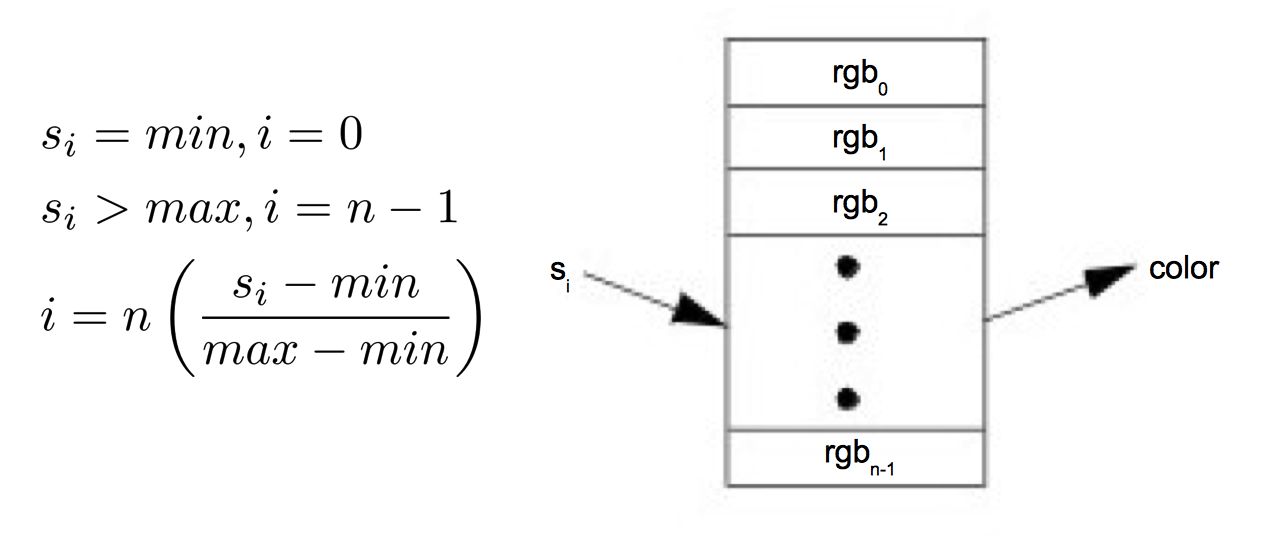
\includegraphics[width=0.8\textwidth]{Figure6-1}\\
	\caption{Mapping scalars to colors via a lookup table.}\label{fig:Figure6-1}
\end{figure}

\section{Generality Versus Efficiency}
Most algorithms can be written specifically for a particular dataset type, or more generally, treating any dataset type. The advantage of a specific algorithm is that it is usually faster than a comparable general algorithm. (See "Other Data Abstractions" on page138 where we discussed the tradeoff between abstract and concrete forms.) An implementation of a specific algorithm also may be more memory efficient and its implementation may better reflect the relationship between the algorithm and the dataset type it operates on.

One example of this is contour surface creation. Algorithms for extracting contour surfaces were originally developed for volume data, mainly for medical applications. The regularity of volumes lends itself to efficient algorithms. However, the specialization of volume-based algorithms precludes their use for more general datasets such as structured or unstructured grids. Although the contour algorithms can be adapted to these other dataset types, they are less efficient than those for volume datasets.

Our presentation of algorithms favors the more general implementations. In some special cases we will describe performance improving techniques for particular dataset types. Refer to the bibliography at the end of each chapter for detailed descriptions of specialized algorithms.

\section{Scalar Algorithms}

Scalars are single data values associated with each point and/or cell of a dataset. (Recall that in the \emph{Visualization Toolkit} we associate data with points.) Because scalar data is commonly found in real-world applications, and because scalar data is so easy to work with, there are many different algorithms to visualize it.

\subsection{Color Mapping}

\emph{Color mapping} is a common scalar visualization technique that maps scalar data to colors, and displays the colors on the computer system. The scalar mapping is implemented by indexing into a \emph{color lookup table}. Scalar values serve as indices into the lookup table.

The mapping proceeds as follows. The lookup table holds an array of colors (e.g., red, green, blue components or other comparable representations). Associated with the table is a minimum and maximum \emph{scalar range (min, max)} into which the scalar values are mapped. Scalar values greater than the maximum range are clamped to the maximum color, scalar values less than the minimum range are clamped to the minimum color value. Then, for each scalar value $x_i$, the index $i$ into the color table with n entries (and 0-offset) is given by Figure \ref{fig:Figure6-1}.

A more general form of the lookup table is called a transfer function. A transfer function is any expression that maps scalar values into a color specification. For example, Figure \ref{fig:Figure6-2} maps scalar values into separate intensity values for the red, green, and blue color components. We can also use transfer functions to map scalar data into other information such as local transparency. (Transfer functions are discussed in more detail in ``Transparency and Alpha Values'' on page \pageref{sec:transparency_alpha} and ``Volume Rendering'' on page \pageref{sec:volume_rendering}).
A lookup table is a discrete sampling of a transfer function.
We can create a lookup table from any transfer function by sampling the transfer function at a set of discrete points.

Color mapping is a one-dimensional visualization technique. It maps one piece of information (i.e., a scalar value) into a color specification. However, the display of color information is not limited to one-dimensional displays. Often we use color information mapped onto 1D, 2D, or 3D objects. This is a simple way to increase the information content of our visualizations.

The key to color mapping for scalar visualization is to choose the lookup table entries carefully. Figure \ref{fig:Figure6-3} shows four different lookup tables used to visualize gas density as fluid flows through a combustion chamber. The first lookup table is gray-scale. Grayscale tables often provide better structural detail to the eye. The other three images in Figure \ref{fig:Figure6-3} uses different colored lookup tables. The second uses rainbow hues from blue to red. The third uses rainbow hues arranged from red to blue. The last table uses a table designed to enhance contrast. Careful use of colors can often enhance important features of a dataset. However, any type of lookup table can exaggerate unimportant details or create visual artifacts because of unforeseen interactions between data, color choice, and human physiology.

Designing lookup tables is as much art as it is science. From a practical point of view, tables should accentuate important features, while minimizing less important or extraneous details. It is also desirable to use palettes that inherently contain scaling information. For example, a color rainbow scale from blue to red is often used to represent temperature scale, since many people associate "blue" with cold temperatures, and "red" with hot temperatures. However, even this scale is problematic: a physicist would say that blue is hotter than red, since hotter objects emit more blue light (i.e., shorter wavelength) than red. Also, there is no need to limit ourselves to "linear" lookup tables. Even though the mapping of scalars into colors has been presented as a linear operation (Figure \ref{fig:Figure6-1}, the table itself need not be linear. That is, tables can be designed to enhance small variations in scalar value using logarithmic or other schemes, improving the comfort level and engaging the human observer more deeply in the presentation of data improves the effectiveness of communication.

\begin{figure}[!htb]
	\centering
	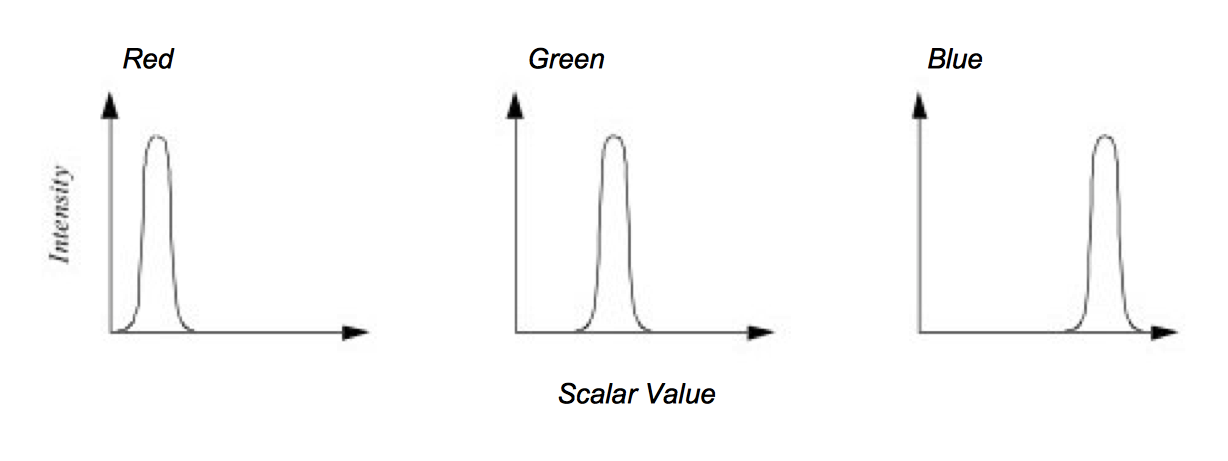
\includegraphics[width=0.8\textwidth]{Figure6-2}
	\caption{Transfer function for color components red, green and blue as a function of scalar value.}
	\label{fig:Figure6-2}
\end{figure}

\begin{figure}[!htb]
	\centering
	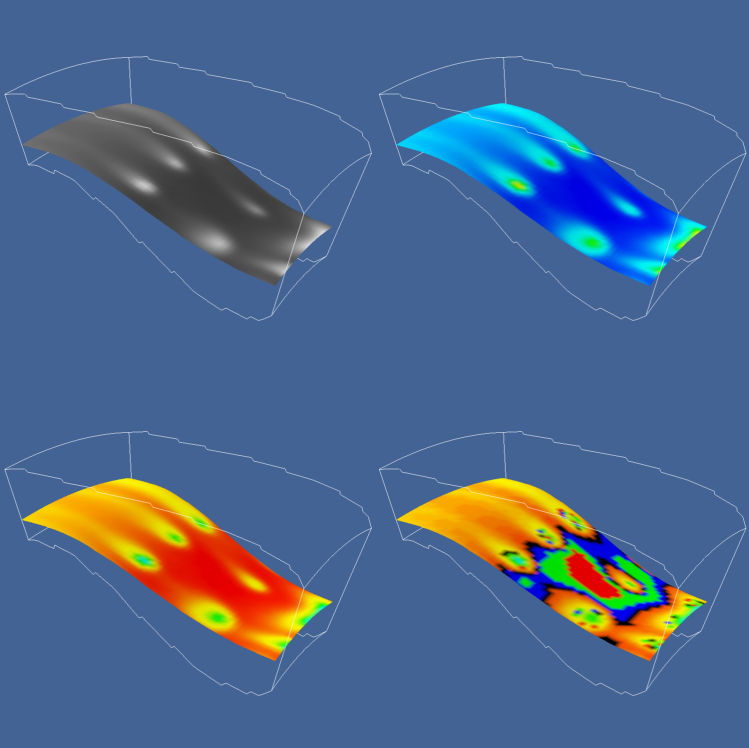
\includegraphics[width=0.8\textwidth]{Figure6-3}
	\caption{Flow density colored with different lookup tables. Top-left: grayscale; Top-right rainbow (blue to red); lower-left rainbow (red to blue); lower-right large contrast. (\href{https://lorensen.github.io/VTKExamples/site/Cxx/Rendering/Rainbow/}{Rainbow.cxx}) and (\href{https://lorensen.github.io/VTKExamples/site/Python/Rendering/Rainbow/}{Rainbow.py})}
	\label{fig:Figure6-3}
\end{figure}

\subsection{Contouring}

A natural extension to color mapping is \emph{contouring}. When we see a surface colored with data values, the eye often separates similarly colored areas into distinct regions. When we contour data, we are effectively constructing the boundary between these regions. These boundaries correspond to contour lines (2D) or surfaces (3D) of constant scalar value.

Examples of 2D contour displays include weather maps annotated with lines of constant temperature (isotherms), or topological maps drawn with lines of constant elevation. Three-dimensional contours are called \emph{isosurfaces}, and can be approximated by many polygonal primitives. Examples of isosurfaces include constant medical image intensity corresponding to body tissues such as skin, bone, or other organs. Other abstract isosurfaces such as surfaces of constant pressure or temperature in fluid flow also may be created.


\begin{figure}[!htb]
	\centering
	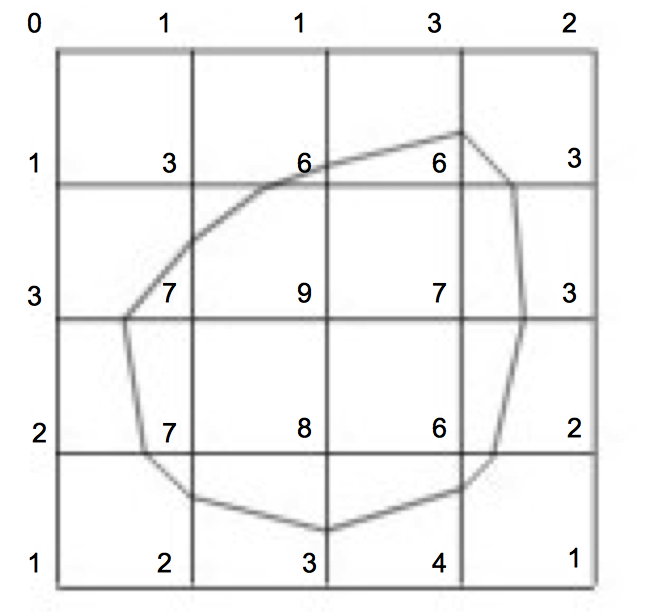
\includegraphics[width=0.8\textwidth]{Figure6-4}
	\caption{ Contouring a 2D stuctured grid with contour line value = 5.}
	\label{fig:Figure6-4}
\end{figure}

Consider the 2D structured grid shown in Figure \ref{fig:Figure6-4}. Scalar values are shown next to the points that define the grid. Contouring always begins by selecting a scalar value, or contour value, that corresponds to the contour lines or surfaces generated. To generate the contours, some form of interpolation must be used. This is because we have scalar values at a finite set of points in the dataset, and our contour value may lie between the point values. Since the most common interpolation technique is linear, we generate points on the contour surface by linear interpolation along the edges. If an edge has scalar values 10 and 0 at its two endpoints, and if we are trying to generate a contour line of value 5, then edge interpolation computes that the contour passes through the midpoint of the edge.

Once the points on cell edges are generated, we can connect these points into contours using a few different approaches. One approach detects an edge intersection (i.e., the contour passes through an edge) and then "tracks" this contour as it moves across cell boundaries. We know that if a contour edge enters a cell, it must exit a cell as well. The contour is tracked until it closes back on itself, or exits a dataset boundary. If it is known that only a single contour exists, then the process stops. Otherwise, every edge in the dataset must be checked to see whether other contour lines exist. Another approach uses a divide and conquer technique, treating cells
independently. This is the \emph{marching squares} algorithm in 2D, and \emph{marching cubes} \cite{Lorensen87} in 3D. The basic assumption of these techniques is that a contour can only pass through a
cell in a finite number of ways. A case table is constructed that enumerates all possible topological \emph{states} of a cell, given combinations of scalar values at the cell points. The number of topological states depends on the number of cell vertices, and the number of inside / outside relationships a vertex can have with respect to the contour value. A vertex is considered inside a contour if its scalar value is larger than the scalar value of the contour line. Vertices with scalar values less than the contour value are said to be outside the contour. For example, if a cell has four vertices and each vertex can be either inside or outside the contour, there are $2^4 = 16$ possible ways that the contour passes through the cell. In the case table we are not interested in where the contour passes through the cell (e.g., geometric intersection), just how it passes through the cell (i.e., topology of the contour in the cell).

Figure \ref{fig:Figure6-5} shows the sixteen combinations for a square cell. An index into the case table can be computed by encoding the state of each vertex as a binary digit. For 2D data represented on a rectangular grid, we can represent the 16 cases with 4 bit index. Once the proper case is selected, the location of the contour line / cell edge intersection can be calculated using interpolation. The algorithm processes a cell and then moves, or \emph{marches t} o the next cell. After all cells are visited, the contour will be completed. In summary, the marching algorithms proceed as follows:

\begin {enumerate}

\item Select a cell.

\item Calculate the inside / outside state of each vertex of the cell.

\item Create an index by storing the binary state of each vertex in a separate bit.

\item Use the index to look up the topological state of the cell in a case
table.

\item Calculate the contour location (via interpolation) for each edge in  the case table.

\end{enumerate}

This procedure will construct independent geometric primitives in each cell. At the cell boundaries duplicate vertices and edges may be created. These duplicates can be eliminated by using a special coincident point merging operation. Note that interpolation along each edge should be done in the same direction. If not, numerical roundoff will likely cause points to be generated that are not precisely coincident, and will not merge properly.

There are advantages and disadvantages to both the edge-tracking and marching cubes approaches. The marching squares algorithm is easy to implement. This is particularly important when we extend the technique into three dimensions, where isosurface tracking becomes much more difficult. On the other hand, the algorithm creates disconnected line segments and points, and the required merging operation requires extra computation resources. The tracking algorithm can be implemented to generate a single polyline per contour line, avoiding the need to merge coincident points.

\begin{figure}[!htb]
\centering
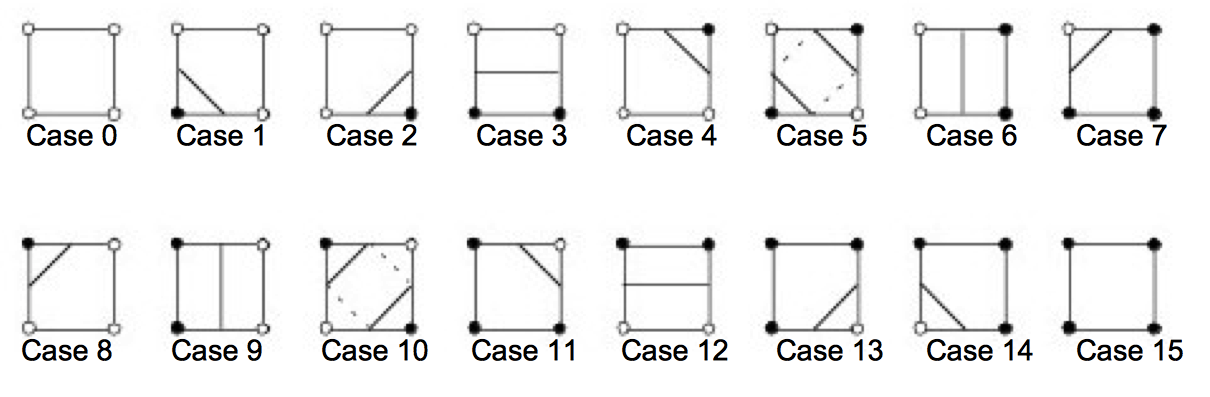
\includegraphics[width=0.8\textwidth]{Figure6-5}\\
\caption{ Sixteen different marching squares cases. Dark vertices indicate scalar value is above contour value. Cases 5 and 10 are ambiguous.}
\label{fig:Figure6-5}
\end{figure}


\begin{figure}[!htb]
	\centering
	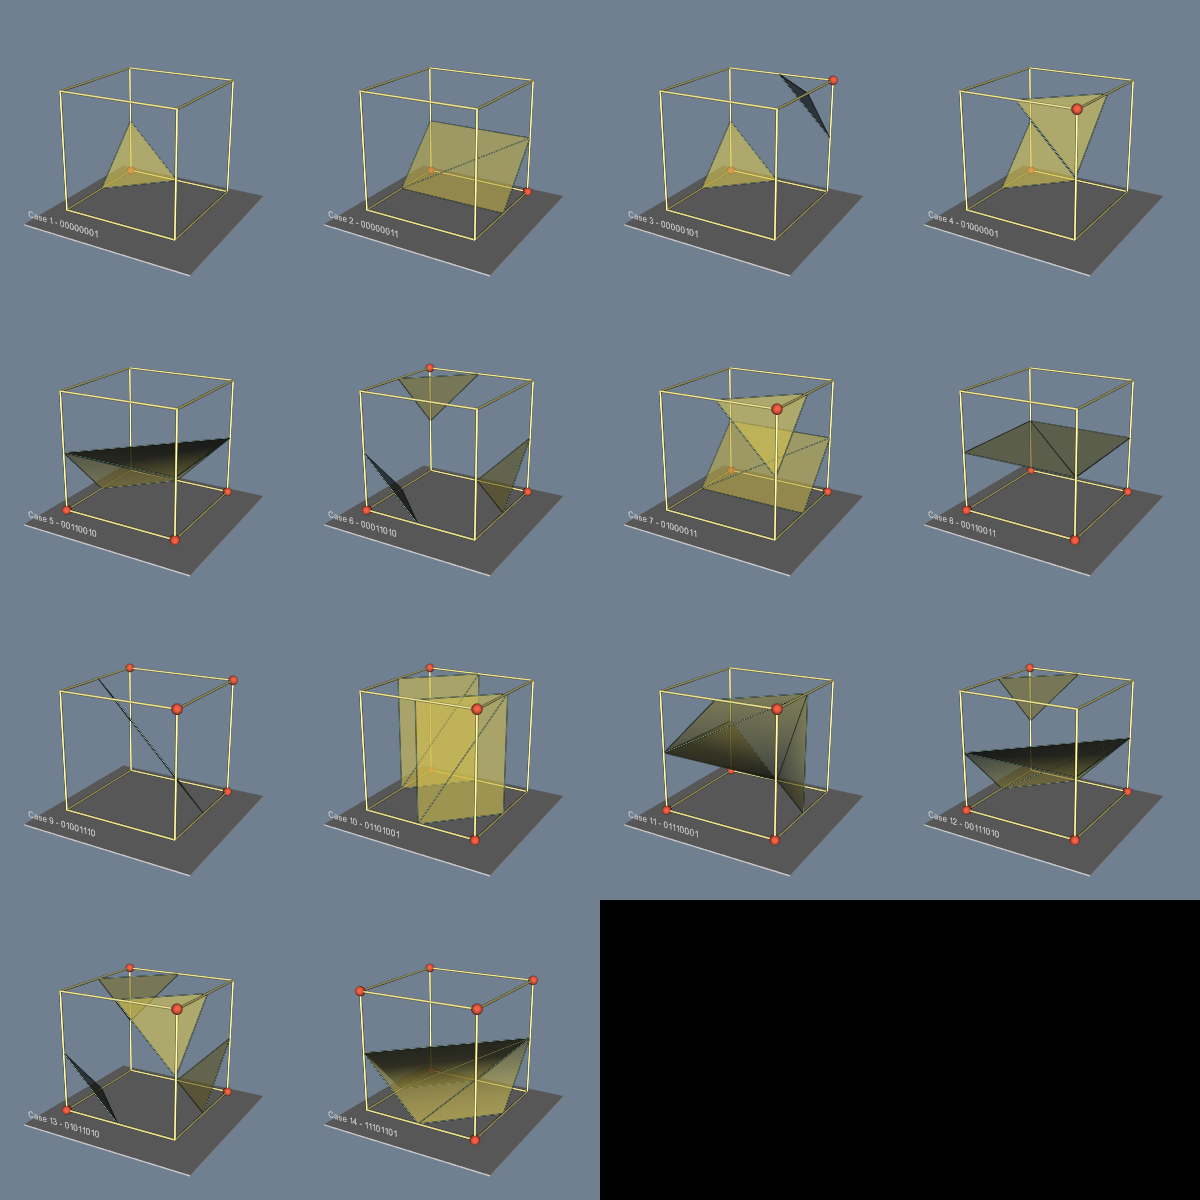
\includegraphics[width=0.8\textwidth]{Figure6-6}\\
	\caption{Marching Cubes cases for 3D isosurface generation. The 256 possible cases have been reduced to 15 cases using symmetry. Red vertices are greater than the selected isosurface value. (\href{https://lorensen.github.io/VTKExamples/site/Cxx/VisualizationAlgorithms/MarchingCasesA/}{MarchingCasesA.cxx}) and (\href{https://lorensen.github.io/VTKExamples/site/Python/VisualizationAlgorithms/MarchingCasesA/}{MarchingCasesA.py})}
	\label{fig:Figure6-6}
\end{figure}


\begin{figure}[!htb]
	\centering
	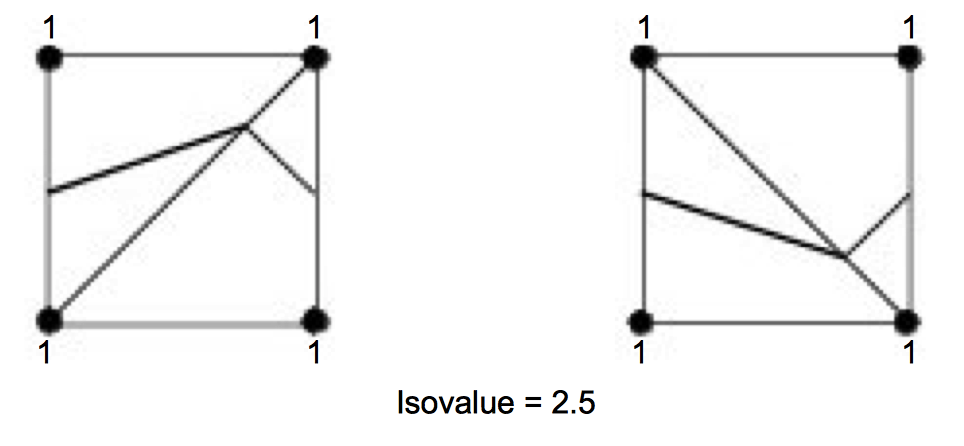
\includegraphics[width=0.8\textwidth]{Figure6-7}\\
	\caption{Using marching triangles or marching tetrahedra to resolve ambiguous cases on rectangular lattice (only face of cube is shown). Choice of diagonal orientation may result in ``bumps'' in contour surface. In 2D, diagonal orientation can be chosen arbitrarily, but in 3D diagonal is constrained by neighbor.}
	\label{fig:Figure6-7}
\end{figure}

As mentioned previously, the 3D analogy of marching squares is marching cubes. Here, there are 256 different combinations of scalar value, given that there are eight points in a cubical cell (i.e., $2^8$ combinations). Figure \ref{fig:Figure6-6} shows these combinations reduced to 15 cases by using arguments of symmetry. We use combinations of rotation and mirroring to produce topologically equivalent cases.

In two dimensions, contour ambiguity is simple to treat: for each ambiguous case we implement one of the two possible cases. The choice for a particular case is independent of all other choices. Depending on the choice, the contour may either extend or break the current contour as illustrated in Figure \ref{fig:Figure6-9}. Either choice is acceptable since the resulting contour lines will be continuous and closed (or will end at the dataset boundary).

In three dimensions the problem is more complex. We cannot simply choose an ambiguous case independent of all other ambiguous cases. For example Figure \ref{fig:Figure6-9} shows what happens if we carelessly implement two cases independent of one another. In this figure we have used the usual case 3 but replaced case 6 with its \emph{complementary} case. Complementary cases are formed by exchanging the ``dark'' vertices with ``light'' vertices. (This is equivalent to swapping vertex scalar value from above the isosurface value to below the isosurface value, and vice versa.) The result of pairing these two cases is that a hole is left in the isosurface.

Several different approaches have been taken to remedy this problem. One approach tessellates the cubes with tetrahedron, and uses a \emph{marching tetrahedra} technique. This works because the marching tetrahedra exhibit no ambiguous cases. Unfortunately, the marching tetrahedra algorithm generates isosurfaces consisting of more triangles, and the tessellation of a cube with tetrahedra requires making a choice regarding the orientation of the tetrahedra. This choice may result in artificial ``bumps'' in the isosurface because of interpolation along the face diagonals as shown in Figure \ref{fig:Figure6-7}. Another approach evaluates the asymptotic behavior of the surface, and then chooses the cases to either join or break the contour. Nielson and Hamann \cite{Nielson91} have developed a technique based on this approach they call the \emph{asymptotic decider}. It is based on an analysis of the variation of the scalar variable across an ambiguous face. The analysis determines how the edges of isosurface polygons should be connected.

\begin{figure}[!htb]
	\centering
	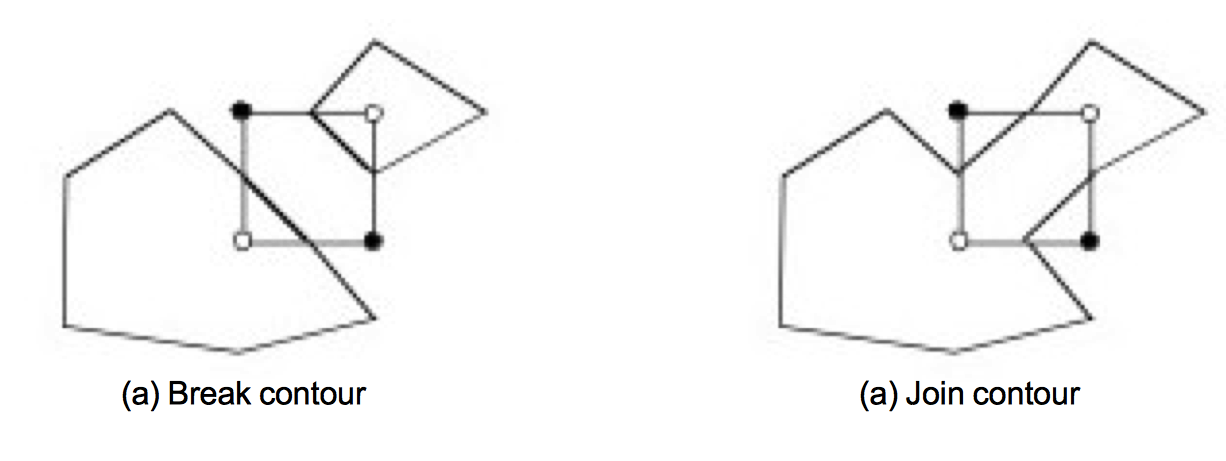
\includegraphics[width=0.8\textwidth]{Figure6-8}\\
	\caption{Choosing a particular contour case will break (a) or join (b) the current contour. Case shown is marching squares case 10.}
	\label{fig:Figure6-8}
\end{figure}

\begin{figure}[!htb]
	\centering
	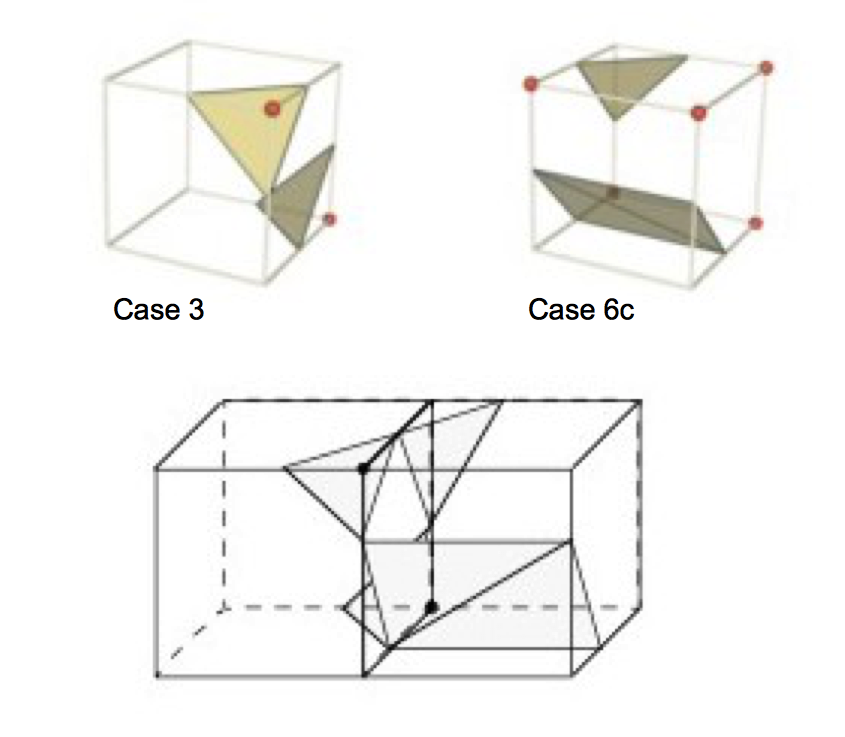
\includegraphics[width=0.8\textwidth]{Figure6-9}\\
	\caption{Arbitrarily choosing marching cubes cases leads to holes in the isosurface.}
	\label{fig:Figure6-9}
\end{figure}

A simple and effective solution extends the original 15 marching cubes cases by adding additional complementary cases. These cases are designed to be compatible with neighboring cases and prevent the creation of holes in the isosurface. There are six complementary cases required, corresponding to the marching cubes cases 3, 6, 7, 10, 12, and 13. The complementary marching cubes cases are shown in Figure \ref{fig:Figure6-10}.

\begin{figure}[!htb]
	\centering
	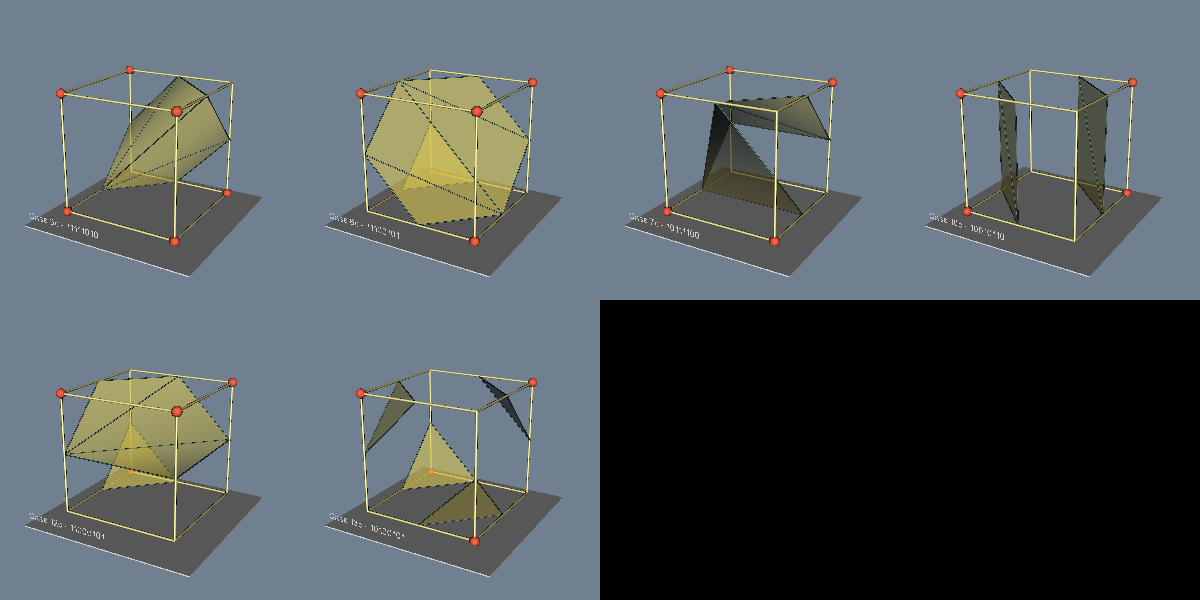
\includegraphics[width=0.8\textwidth]{Figure6-10}\\
	\caption{Marching cubes complementary cases.(\href{https://lorensen.github.io/VTKExamples/site/Cxx/VisualizationAlgorithms/MarchingCasesB/}{MarchingCasesB.cxx}) and (\href{https://lorensen.github.io/VTKExamples/site/Python/VisualizationAlgorithms/MarchingCasesB/}{MarchingCasesB.py})}
	\label{fig:Figure6-10}
\end{figure}

We can extend the general approach of marching squares and marching cubes to other topological types. In VTK we use marching lines, triangles, and tetrahedra to contour cells of these types (or composite cells that are composed of these types). In addition, although we speak of regular types such as squares and cubes, marching cubes can be applied to any cell type topologically equivalent to a cube (e.g., hexahedron or non-cubical voxel).

Figure \ref{fig:Figure6-11} shows four applications of contouring. In Figure \ref{fig:Figure6-11a} we see 2D contour lines of CT density value corresponding to different tissue types. These lines were generated using marching squares. Figure \ref{fig:Figure6-11b} through Figure \ref{fig:Figure6-11d} are isosurfaces created by marching cubes. Figure \ref{fig:Figure6-11b} is a surface of constant image intensity from a computed tomography (CT) Xray imaging system. ( Figure \ref{fig:Figure6-11a} is a 2D subset of this data.) The intensity level corresponds to human bone. Figure \ref{fig:Figure6-11c} is an isosurface of constant flow density. Figure \ref{fig:Figure6-11d} is an isosurface of electron potential of an iron protein molecule. The image shown in Figure \ref{fig:Figure6-11b} is immediately recognizable because of our familiarity with human anatomy. However, for those practitioners in the fields of computational fluid dynamics and molecular biology, Figure \ref{fig:Figure6-11c} and Figure \ref{fig:Figure6-11d} are equally familiar. As these examples show, methods for contouring are powerful yet general techniques for visualizing data from a variety of fields.

\begin{figure}
	\begin{subfigure}[h]{0.48\linewidth}
		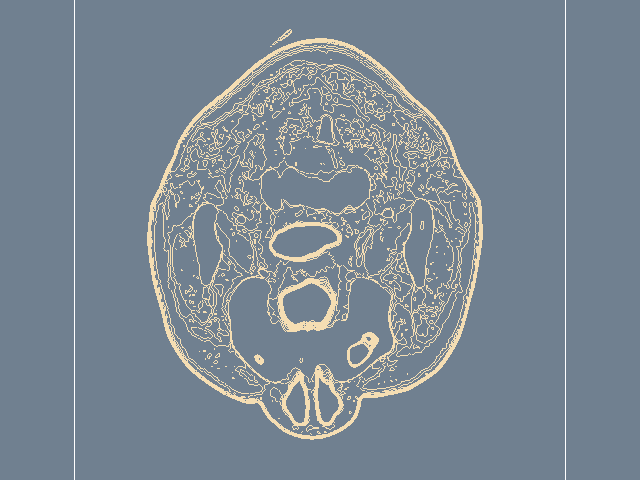
\includegraphics[width=\linewidth]{Figure6-11a}
		\caption{Marching squares used to generate contour lines.(\href{https://lorensen.github.io/VTKExamples/site/Cxx/VisualizationAlgorithms/HeadSlice}{HeadSlice.cxx} or \href{https://lorensen.github.io/VTKExamples/site/Python/VisualizationAlgorithms/HeadSlice/}{HeadSlice.py})}\label{fig:Figure6-11a}
	\end{subfigure}
	\hfill
	\begin{subfigure}[h]{0.48\linewidth}
		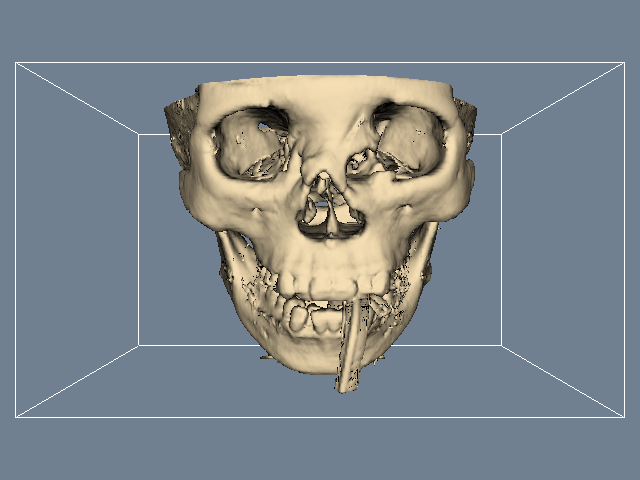
\includegraphics[width=\linewidth]{Figure6-11b}
		\caption{Marching Cubes surface of human bone.(\href{https://lorensen.github.io/VTKExamples/site/Cxx/VisualizationAlgorithms/HeadBone}{HeadBone.cxx} or \href{https://lorensen.github.io/VTKExamples/site/Python/VisualizationAlgorithms/HeadBone/}{HeadBone.py})}\label{fig:Figure6-11b}
	\end{subfigure}%
	\hfill
	\begin{subfigure}[h]{0.48\linewidth}
		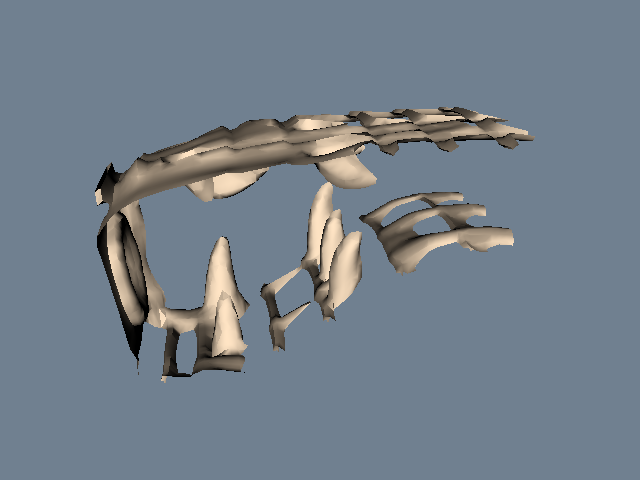
\includegraphics[width=\linewidth]{Figure6-11c}
		\caption{Marching squares used to generate contour lines.(\href{https://lorensen.github.io/VTKExamples/site/Cxx/VisualizationAlgorithms/CombustorIsosurface}{CombustorIsosurface.cxx} or \href{https://lorensen.github.io/VTKExamples/site/Python/VisualizationAlgorithms/CombustorIsosurface/}{CombustorIsosurface.py})}\label{fig:Figure6-11c}
	\end{subfigure}
	\hfill
	\begin{subfigure}[h]{0.48\linewidth}
		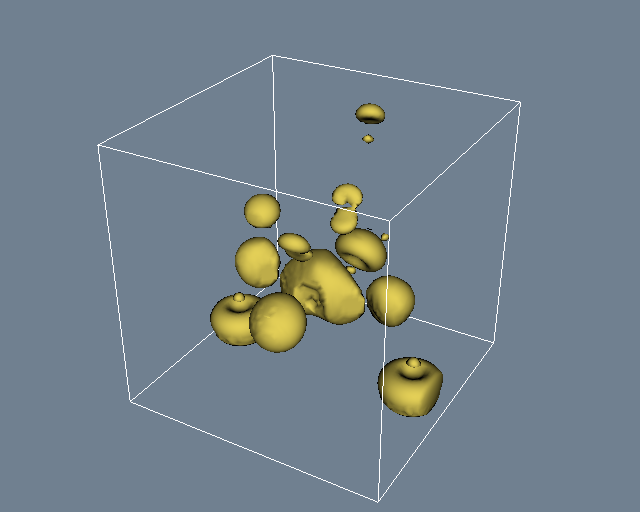
\includegraphics[width=\linewidth]{Figure6-11d}
		\caption{Marching Cubes surface of human bone.(\href{https://lorensen.github.io/VTKExamples/site/Cxx/VisualizationAlgorithms/IronIsoSurface}{IronIsoSurface.cxx} or \href{https://lorensen.github.io/VTKExamples/site/Python/VisualizationAlgorithms/IronIsoSurface/}{IronIsoSurface.py})}\label{fig:Figure6-11d}
	\end{subfigure}%
	\caption{Contouring examples.}\label{fig:Figure6-11}
\end{figure}

\subsection{Scalar Generation}

The two visualization techniques presented thus far, color mapping and contouring, are simple, effective methods to display scalar information. It is natural to turn to these techniques first when visualizing data. However, often our data is not in a form convenient to these techniques. The data may not be single-valued (i.e., a scalar), or it may be a mathematical or other complex relationship. That is part of the fun and creative challenge of visualization: We must tap our creative resources to convert data into a form we can visualize.

For example, consider terrain data. We assume that the data is \emph{xyz} coordinates, where \emph{x} and \emph{y} represent the coordinates in the plane, and \emph{z} represents the elevation above sea level. Our desired visualization is to color the terrain according to elevation. This requires creating a color map --- possibly using white for high altitudes, blue for sea level and below, and various shades of green and brown corresponding to elevation between sea level and high altitude. We also need scalars to index into the color map. The obvious choice here is to extract the \emph{z} coordinate. That is, scalars are simply the \emph{z}-coordinate value.

This example can be made more interesting by generalizing the problem. Although we could easily create a filter to extract the \emph{z}-coordinate, we can create a filter that produces elevation scalar values where the elevation is measured along any axis. Given an oriented line starting at the (low) point $p_l$ (e.g., sea level) and ending at the (high) point $p_h$ (e.g., mountain top), we compute the elevation scalar $s_i$ at point $p_i = (x_i, y_i,z_i)$ using the dot product as shown in Figure \ref{fig:Figure6-12}. The scalar is normalized using the magnitude of the oriented line, and may be clamped between minimum and maximum scalar values (if necessary). The bottom half of this figure shows the results of applying this technique to a terrain model of Honolulu, Hawaii. A lookup table of 256 colors ranging from deep brown (water) to dark turquoise (mountain top) is used to color map this figure.

\begin{figure}
	\begin{subfigure}[h]{0.96\linewidth}
		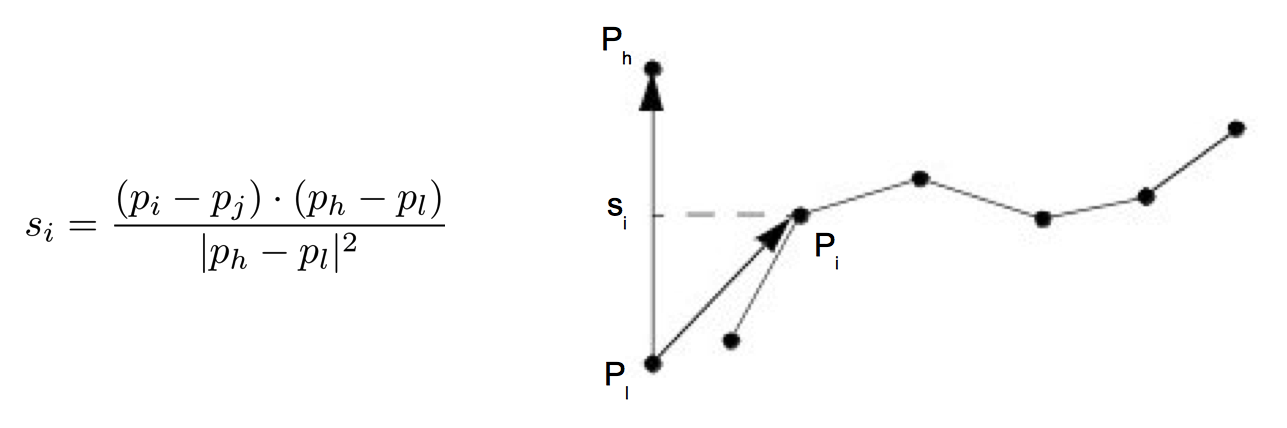
\includegraphics[width=\linewidth]{Figure6-12a}
	\end{subfigure}
	\hfill
	\begin{subfigure}[h]{0.48\linewidth}
		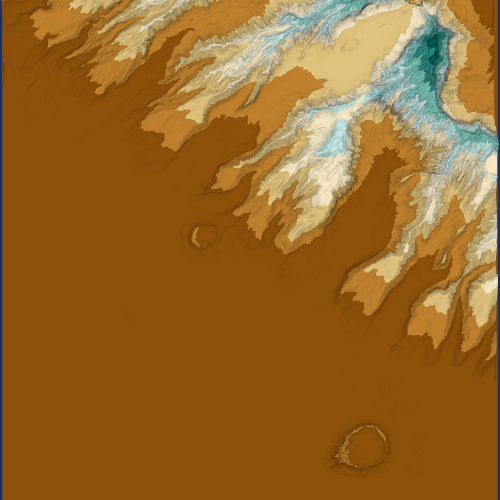
\includegraphics[width=\linewidth]{Figure6-12b}
		\caption*{Applying the technique to terrain data from Honolulu, Hawaii.(\href{https://lorensen.github.io/VTKExamples/site/Cxx/Visualization/Hawaii}{Hawaii.cxx} or \href{https://lorensen.github.io/VTKExamples/site/Python/Visualization/Hawaii/}{Hawaii.py})}
	\end{subfigure}%
	\caption{Computing scalars using normalized dot product.}\label{fig:Figure6-12}
\end{figure}

Part of the creative practice of visualization is selecting the best technique for given data from the palette of available techniques. Often this requires creative mapping by the user of the visualization system. In particular, to use scalar visualization techniques we need only to create a relationship to generate a unique scalar value. Other examples of scalar mapping include an index value into a list of data, computing vector magnitude or matrix determinate, evaluating surface curvature, or determining distance between points. Scalar generation, when coupled with color mapping or contouring, is a simple, yet effective, technique for visualizing many types of data.

\section{Vector Algorithms}

Vector data is a three-dimensional representation of direction and magnitude. Vector data often results from the study of fluid flow, or when examining derivatives (i.e., rate of change) of some quantity.

\subsection{Hedgehogs and Oriented Glyphs}

A natural vector visualization technique is to draw an oriented,
scaled line for each vector (Figure \ref{fig:Figure6-13a}). The line begins at the point with which the vector is associated and is oriented in the direction of the vector components $(v_x, v_y, v_z)$. Typically, the resulting line must be scaled up or down to control the size of its visual representation. This technique is often referred to as a *hedgehog* because of the bristly result.

There are many variations of this technique Figure \ref{fig:Figure6-13b}). Arrows may be added to indicate the direction of the line. The lines may be colored according to vector magnitude, or some other scalar quantity (e.g., pressure or temperature). Also, instead of using a line, oriented ``glyphs'' can be used. By glyph we mean any 2D or 3D geometric representation such as an oriented triangle or cone.

\begin{figure}
	\begin{subfigure}[h]{0.24\linewidth}
		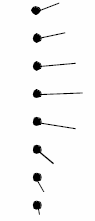
\includegraphics[width=\linewidth]{Figure6-13a}
		\caption{Oriented lines.}\label{fig:Figure6-13a}
	\end{subfigure}
	\hfill
	\begin{subfigure}[h]{0.24\linewidth}
		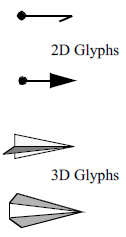
\includegraphics[width=\linewidth]{Figure6-13b}
		\caption{Glyphs}\label{fig:Figure6-13b}
	\end{subfigure}%
	\hfill
	\begin{subfigure}[h]{0.48\linewidth}
		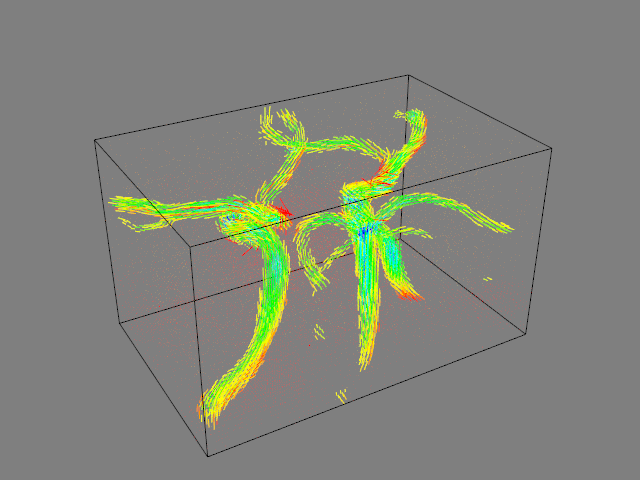
\includegraphics[width=\linewidth]{Figure6-13c}
		\caption{Complex vector visualization. (\href{https://lorensen.github.io/VTKExamples/site/Cxx/Visualization/TestComplexV}{TestComplexV.cxx} or \href{https://lorensen.github.io/VTKExamples/site/Python/Visualization/TestComplexV/}{TestComplexV.py})}\label{fig:Figure6-13c}
	\end{subfigure}
	\caption{Vector visualization techniques.}\label{fig:Figure6-13}
\end{figure}

Care should be used in applying these techniques. In 3D it is often difficult to understand the position and orientation of a vector because of its projection into a 2D image. Also, using large numbers of vectors can clutter the display to the point where the visualization becomes meaningless. Figure \ref{fig:Figure6-13c} shows 167,000 3D vectors (using oriented and scaled lines) in the region of the human carotid artery. The larger vectors lie inside the arteries, the smaller vectors lie outside the arteries and are randomly oriented (measurement error) but small in magnitude. Clearly the details of the vector field are not discernible from this image.

Scaling glyphs also poses interesting problems. In what Tufte has termed a ``visualization lie'', \cite{Tufte83} scaling a 2D or 3D glyph results in nonlinear differences in appearance. The surface area of an object increases with the square of its scale factor, so two vectors differing by a factor of two in magnitude may appear up to four times different based on surface area. Such scaling issues are common in data visualization, and great care must be taken to avoiding misleading viewers.

\subsection{Warping}

Vector data is often associated with ``motion''. The motion is in the form of velocity or displacement. An effective technique for displaying such vector data is to ``warp'' or deform geometry according to the vector field. For example, imagine representing the displacement of a structure under load by deforming the structure. Or if we are visualizing the flow of fluid, we can create a flow profile by distorting a straight line inserted perpendicular to the flow.
\section{Bibliographic Notes}

Color mapping is a widely studied topic in imaging, computer graphics, visualization, and human factors. References \cite{Durrett87} \cite{Ware88} \cite{Rheingans92} provide samples of the available literature. You also may want to learn about the physiological and psychological effects of color on perception. The text by Wyszecki and Stiles \cite{Wyszecki82} serves as an introductory reference.

Contouring is a widely studied technique in visualization because of its importance and popularity. Early techniques were developed for 2D data \cite{Watson92}. Three-dimensional techniques were developed initially as contour connecting methods \cite{Fuchs77} --- that is, given a series of 2D contours on evenly spaced planes, connect the contours to create a closed surface. Since the introduction of marching cubes \cite{Lorensen87}, many other techniques have been implemented. (A few of these include \cite{Nielson91} \cite{Montani94} and \cite{Durst88} ). A particularly interesting reference is given by Livnat et al. \cite{Livnat96}. They show a contouring method with the addition of a preprocessing step that generates isocontours in near optimal time.

Although we barely touched the topic, the study of chaos and chaotic vibrations is a delightfully interesting topic. Besides the original paper by Lorenz \cite{Lorenz63}, the book by Moon \cite{Moon87} is a good place to start.

Two- and three-dimensional vector plots have been used by computer analysts for many years \cite{Fuller80}. Streamlines and streamribbons also have been applied to the visualization of complex flows \cite{Volpe89}. Good general references on vector visualization techniques are given in \cite{Helman90} and \cite{Richter90}.

Tensor visualization techniques are relatively few in number. Most techniques are glyph oriented \cite{Haber90} \cite{deLeeuw93}. We will see a few more techniques in Chapter 9.

Blinn \cite{Blinn82}, Bloomental \cite{Bloomenthal88} \cite{Bloomenthal97} and Wyvill \cite{Wyvill86} have been important contributors to implicit modeling. Implicit modeling is currently popular in computer graphics for modeling ``soft'' or ``blobby'' objects. These techniques are simple, powerful, and are becoming widely used for advanced computer graphics modeling.


\printbibliography


\section{Exercises}
\begin{enumerate}

\item Sketch contour cases for marching triangles. How many cases are there?

\item Sketch contour cases for marching tetrahedron. How many cases are there?

\item A common visualization technique is to animate isosurface value. The procedure is to smoothly vary isosurface value over a specified range.	
\begin{enumerate}
	\item Create an animation sequence for the quadric example ( **Figure4--1** )
	\item Create an animation sequence for the head sequence ( **Figure6-11** (b))
\end{enumerate}

\item Marching Cubes visits each cell during algorithm execution. Many of these cells do not contain the isosurface. Describe a technique to improve the performance of isosurface extraction by eliminating visits to cells not containing isosurface. ( \emph{Hint}: use a preprocessing step to analyze data. Assume that many isosurfaces will be extracted and that the preprocessing step will not count against execution time.)

\item Scanline rasterization proceeds along horizontal spans in graphics hardware (see ``Rasterization'' on page \pageref{subsec:rasterization}. Interpolation of color occurs along horizontal spans as well.
\begin{enumerate}
	\item Show how the orientation of a polygon affects interpolated color.
	\item Discuss potential problems caused by orientation dependent viewing of visualizations.
\end{enumerate}

\item Write a program to simulate beam vibration. Use the code associated with **Figure6-14** (a) as your starting point.

\item 	 Using the filters vtkStreamLine, vtkMaskPoints, and vtkGlyph3D, create a visualization consisting of oriented glyphs along a streamline.

\item Visualize the following functions.
\begin{enumerate}
	\item Scalar $S(x,y,z)=sin(xy)$ for $x,y$, between $0$ and $\pi$.
	\item The effective stress field (a scalar field) from **Figure6–21**.
	\item The vector field described in the combustor data (i.e., combq.bin and combxyz.bin ).
\end{enumerate}

\item Tensor ellipsoids are based on an ellipsoidal glyph. Describe two other glyphs that you might use.

\item Write a source object to generate a polygonal representation of a torus.

\item Design a glyph to convey airplane heading, speed, and altitude, and proximity (i.e., distance) to other planes.

\item Morphing is a process to smoothly blend images (2D) or geometry (3D) between two known images or geometry. Using an implicit modeling approach, how would you morph a torus into a cube?

\item Describe a technique to visualize vector information by animating a color map. (emph{Hint:} By choosing a map carefully, you can give the illusion of motion across a surface.)

\item Isoline contours of different values are typically shown together in one image.
\begin{enumerate}
	\item Describe the advantages and disadvantages of displaying isosurfaces simultaneously.
	\item What two graphics properties might you adjust to improve the display of multiple isosurefaces?
\end{enumerate}

\item Describe a parallel algorithm for marching cubes. Use a parallel architecture of your choice.

\item Decomposition can greatly increase the speed of an operation.
\begin{enumerate}
	\item  Prove that 3D Gaussian smoothing can be decomposed into three 1D operations.
	\item Give the complexity of the decomposed filter and the same filter implemented as a 3D convolution.
	\item Under what conditions can constant smoothing be decomposed into 1D operations.
\end{enumerate}

\end{enumerate}
